\documentclass{MNR}
%\setcounter{page}{}
%\journaltitle{}
%\volume{}
%\pubyear{}
%\doi{}
%\articlenumber{}
%\articletype{}


\articletitle{} % To break lines in long titles use \\
%%%%%%%%%%%%%%%%%%%%%%%%%%%%%%%%%%%%%%%%%%%%%%%%%%%%%%%%
%%%
%%%  Main document.
%%%
%%%  To span floating objects (wide images, tables, etc.)
%%%  over twocolumn layout, use figure*
%%%  or table* environments.
%%%
%%%  Examples:
%%%  \begin{figure*}	 \begin{table*}		
%%%   ...				  ...				
%%%  \end{figure*}		 \end{table*}		
%%%
%%%%%%%%%%%%%%%%%%%%%%%%%%%%%%%%%%%%%%%%%%%%%%%%%%%%%%%%
\begin{document}
\maketitle 
\section*{Preparation of blood clots}
An aliquot of blood enough to fill a red top vacutainer was drawn from three donors (the Authors male 25 yrs, male 23 yrs and male 21 yrs) for each sample run. The vacutainer was then incubated at 37  $37\,^{\circ}{\rm C}$. in controlled temperature water bath for 1 hour. The blood coagulated to form a mother clot with a long columnar shape. To get rid of the adherent serum off the clot, it was laid on plastic paraffin film and roll dried for 50 cm, left for 5 minutes to air dry, then further roll dried for 50 cm. The mother clot was then cut into daughter clots of ~ 3 mm length each, which each daughter clot was roll dried for 30 cm four times with 1 minute pause interval between each time for air drying. A 20 cm segment was cut from an infusion set tube with 3 mm inner diameter to mimic a human blood vessel. The daughter clot was then loaded into the infusion set segment by sticking it on the tube opening and then centered in the segment by gentle air blowing. The infusion set segment-blood clot system was then filled proximally and distally with Phosphate Buffer Saline by using a 5 mL syringe (gauge 22 needle) through the infusion set segment wall. The tube ends were closed using adhesive gum (Blu-tack)

\section*{Experiment parameters}

\subsection*{Medium parameters}
The medium used was phosphate buffer saline(PBS), because we think it would be closer to mimicking the blood's rate of dissolution,  but it doesnt mimic the blood's viscosity, the blood has a viscosity of 3-4 mPaS while the PBS has a viscosity of of 1.05 mPaS (the robot propels itself better in the blood's viscosity because of the lower reynold's number).

\subsection*{Blood clot parameters}
A volume of 5mL of blood was drawn from abdelrahman (male 25 yrs) to form the mother clot. The vacutainer was taken out of the water bath after 1 hours to begin roll drying. The infusion set-daughter clot system preparation took 90 minutes.



\subsection*{Drilling parameters}
The experiment was done with an angular speed of 6 Hz(one motor at 6 Hz, the other one is around 6 Hz), and a center to center distance of between both end effectors 15 cm along the x-axis at the center. the end effectors were shifted along the z-axis by 2 cm, applying a field of 17.1 mT and a magnetic field gradient of 0.36 mT/mm.

\begin{figure}[t]
\centering
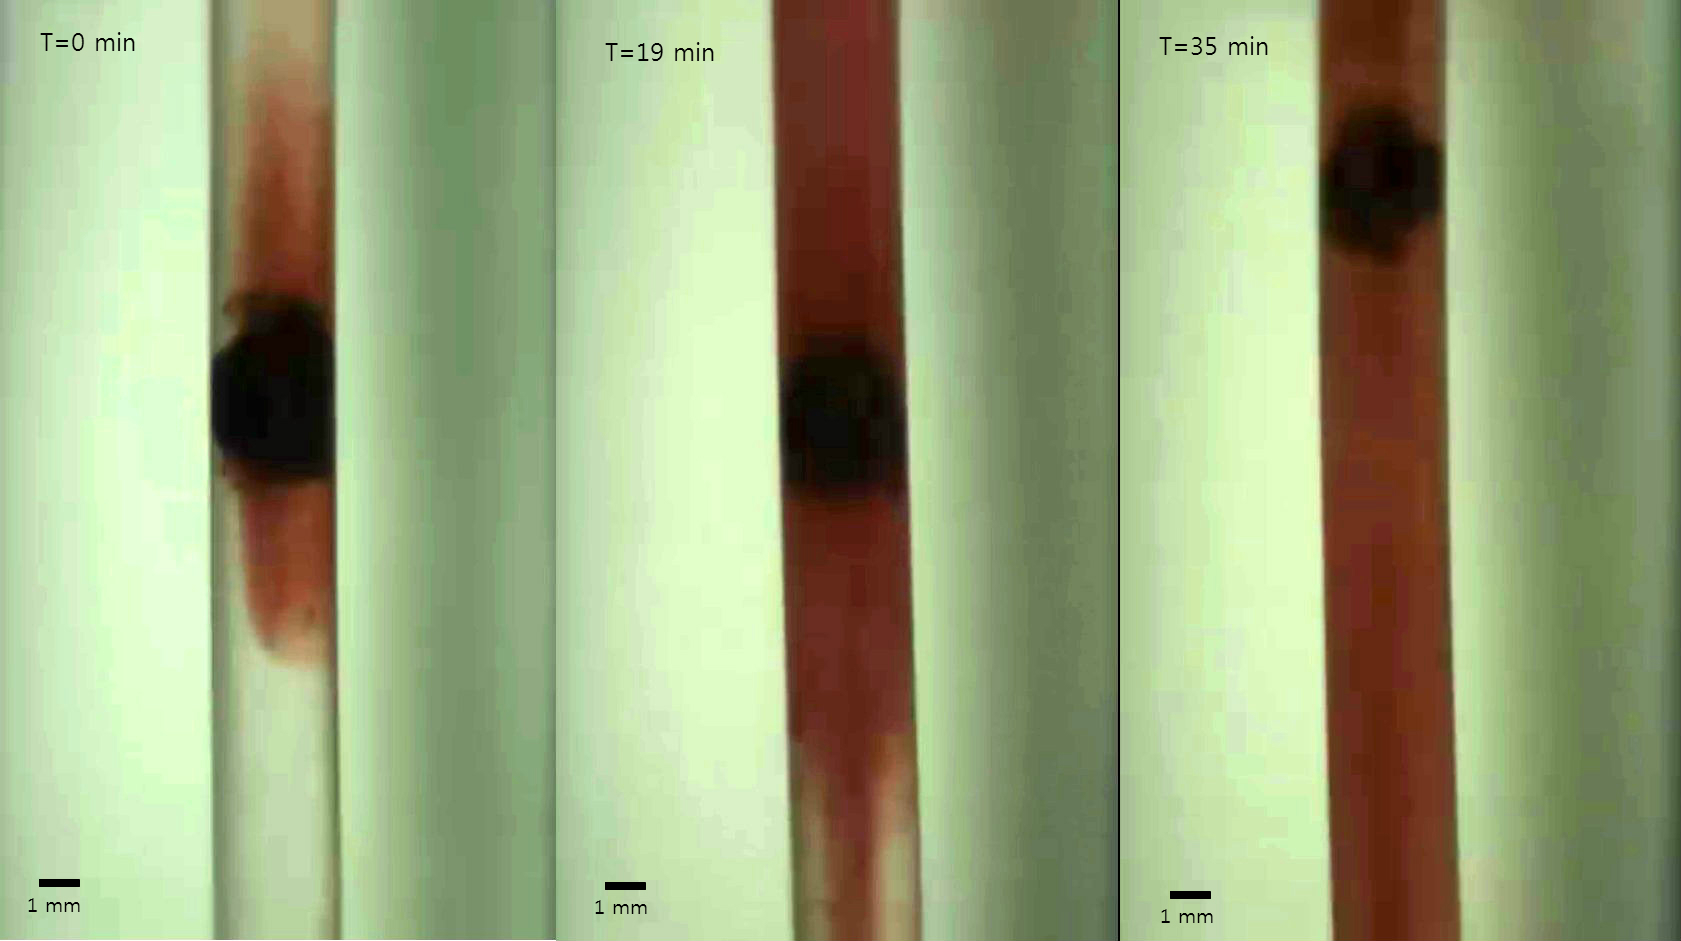
\includegraphics[width=3.2in]{13-7exp-edit}
\caption{The change of the blood clot during the experiment, it can be`noted that the blood clot was reduced in size, as some of its constituents has dissolved in the medium (PBS).  }\label{fig01:System}
\end{figure}

\begin{equation} 
F_t(P)=(M_t.\nabla)B_t(P)
\end{equation} 
The thrust force applied during drilling was applied from the magnetic force $F_t(P)$  where the magnetization of the helical microrobot is noted as $M_t$, and the magnetic field is noted as $B_t$ and $\nabla$ is the gradient operator.

\begin{equation} 
T_t(P)=M_t\times B_t(P)
\end{equation}
The drilling torque $T_t$ is applied from the rotating magnetic field (with a Magnetic field strength of 17.2 mT) from the rotating end effectors



\section*{Results}
\subsection*{Drilling strategy}
The robot started out by drilling away the weaker parts of the blood clot, then we attempted to drill the robot into the blood clot, which is when we realized that we were capable of rotating the blood clot with the rotating magnetic field, it first started with rotating it very slowly due to the strong adhesion forces between the blood clot and the walls of the tube, after the robot was able to weaken the adhesion force, it was able to rotate the blood clot at a much faster rate.

\subsection*{adhesion}


\begin{figure}[h]
\centering
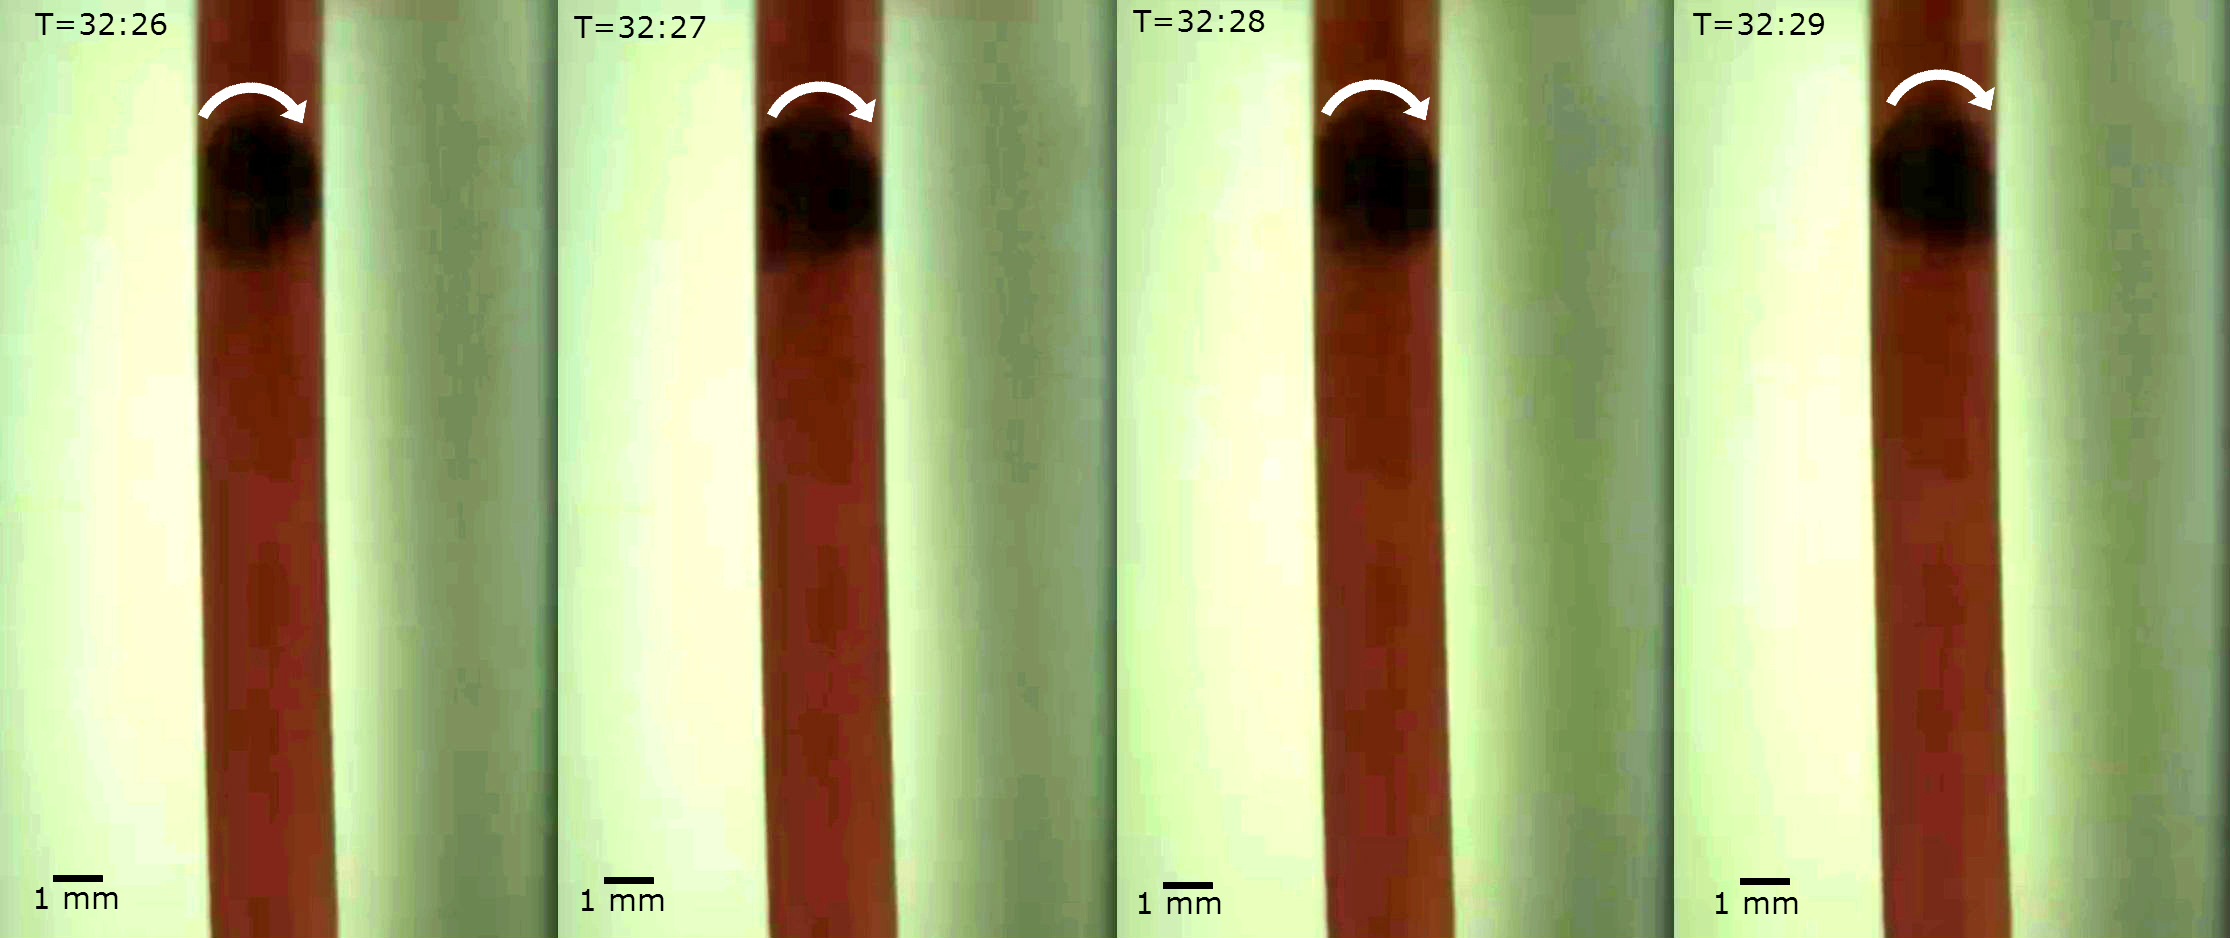
\includegraphics[width=3.2in]{rotclotedit}
\caption{After the microrobot successfully drilled itself into the blood clot it broke the adhesion between the blood clot and the wall by slowly rotating the whole clot }\label{fig01:System}
\end{figure}

\subsection*{Image processing}
An image processing code was written to detect the blood clot in the image and calculate it's size, the process is explained in the previous report "Evaluation of blood clots using image processing"
\begin{figure}[h]
\centering
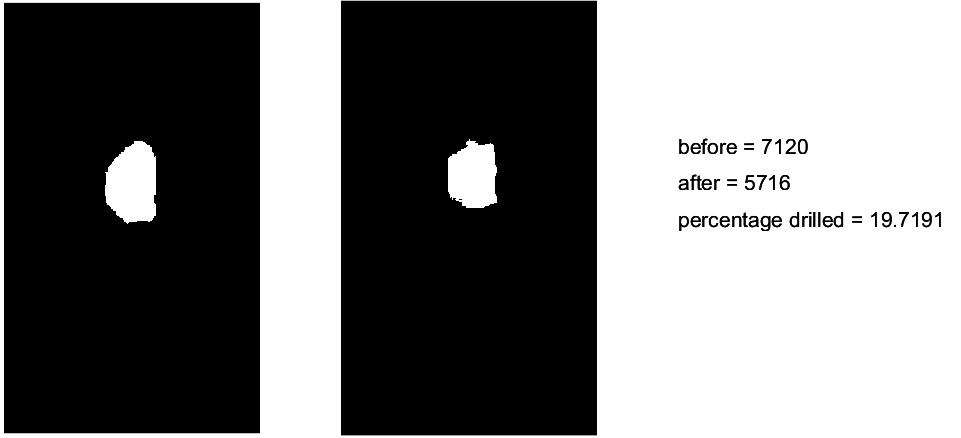
\includegraphics[width=3.2in]{myfig}
\caption{The change in blood clot size and shape after 20 minutes of drilling }\label{fig01:System}
\end{figure}
We then processed the video of the experiment to record the change of the blood clot size with time, and it can be observed it's almost a linear relationship between the decay of the blood clot's size with time, during drilling.
\begin{figure}[h]
\centering
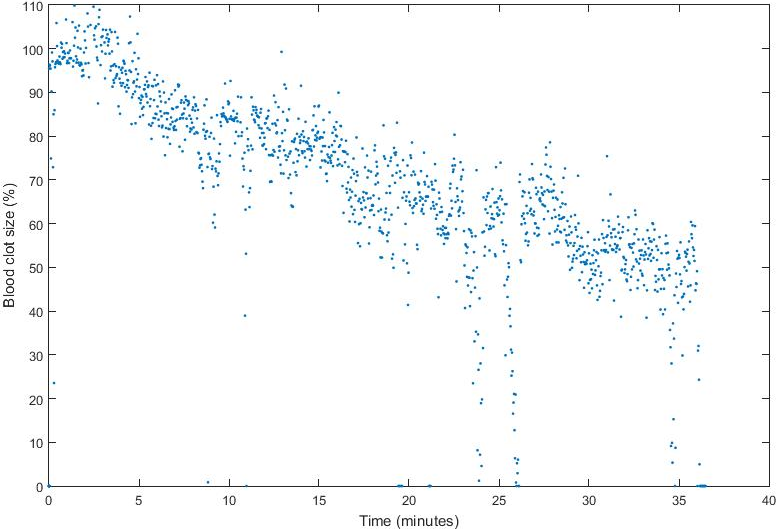
\includegraphics[width=3.2in]{graph3}
\caption{The decay of the blood clot over time }\label{fig01:System}
\end{figure}

\section*{Remarks}
\subsection*{Preparation of blood clots}
Daughter clots should be cut from the mother clot one daughter at a time and the mother is left in its serum to avoid over drying. After roll drying of the daughter clots they should be inserted immediately in the catheter to avoid excessive air drying of the blood clots.The blood clot should stay "30 minutes" in the catheter before injecting PBS in order to avoid mixing of the clot constituents with the fluid before starting the drilling procedure. 



\subsection*{Setup}
The lighting in the experiment needs to be controlled, as it does affect the accuracy of the blood clot measurements; lighting from the sides should be blocked to prevent the shadows being applied from the end effectors, lighting needs to be applied from inside of the setup.
One of the maxon motors needs to be replaced because of a broken encoder, it would give a more powerful synchronous drilling torque.



\begin{thebibliography}{500} % Include .bib (.bbl) references here

\bibitem{Hoffman}
Andrew~Hoffman,~and~Harjit~Gill~"Diastolic timed vibro-percussion at 50Hz delivered across a chest wall sized meat barrier enhances clot dissolution and remotely administered streptokinase effectiveness in an in-vitro model of acute coronary thrombosis" \emph{Thrombosis Journal},10:23, 2012.



\end{thebibliography}

\end{document}